\section{Empirical Checks of the Terms of the Main Bound}
\label{app:beyond}
\providecommand{\ontoR}{\raggedright\hspace{0pt}}
\renewcommand{\topfraction}{0.9}\renewcommand{\textfraction}{0.08}\renewcommand{\floatpagefraction}{0.85}

On Countdown, the projection $\Phi$ of Theorem~\ref{thm:unified_bound} maps a trajectory to the twelve coordinates $\boldsymbol\chi$ of Appendix~\ref{app:trajectory-space}. Appendix~\ref{app:ontology} derives the requirements that the terms of the bound place on the coordinates of a projection. We then report eight experiments that we designed, each of which concerns one part of the bound. Experiment~1 examines whether more coordinates improve the projection on Countdown. Experiments~2 and~3 ask whether $\widehat W_1$ separates groups of agent, embodied and robot trajectories whose tasks differ in structure, and whether a change of agent program alone shifts the trajectories and the success of one model (Appendix~\ref{app:c2}). Experiments~4--6 test Lemma~\ref{lemma:ape_shattering}, the basis of the factor $K_{f,\mathrm{PE}}$, on attention scores, on answers under shifted position indices and on two Countdown models (Appendix~\ref{app:c1}). Experiments~7 and~8 concern the depth term and whether splitting a deeply nested task into separate model calls restores the success that one call loses (Appendix~\ref{app:handoff}). The code repository (\url{https://github.com/Yyuzrah/AMTA4R}) holds the code, all per-pair, per-model and per-run results, and a catalogue of candidate coordinates for Countdown and six other trajectory domains.

\subsection{How the Coordinates of \texorpdfstring{$\Phi$}{Phi} Are Chosen}
\label{app:ontology}

A projection $\Phi_D$ for a trajectory domain $D$ maps a trajectory to $d_\Phi$ coordinates. The upper bound of Theorem~\ref{thm:unified_bound} adds to the source risk the shift term $K_{f,\mathrm{PE}}W_1(\nu_S,\nu_T)$ and twice the residual $\epsilon$ of Assumption~\ref{assum:epsilon_relaxed}, where $\nu_S$ and $\nu_T$ are the distributions of $\Phi(z)$ on the source and target tasks and $K_{f,\mathrm{PE}}$ is the Lipschitz constant of the risk as a function of $\Phi(z)$. The lower bound is the largest of three terms: the source risk minus the shift term and $2\epsilon$, a width term $C_{\mathrm{width}}/\sqrt m-\epsilon$ for a model of width $m$, and a depth term $C_{\mathrm{depth}}\int P_{\mathrm{implicit}}\,d\nu_T-\epsilon$. Every term except the width term places a requirement on the coordinates, and so does the estimation of $W_1$ from samples. We state these requirements in terms of events, the steps of a trajectory, such as the actions and observations of an agent or the visited nodes of a Countdown search.

The residual $\epsilon$ accounts for what $\Phi(z)$ leaves out, such as the operand values of a Countdown problem (Appendix~\ref{app:empirical_sufficiency}). A coordinate therefore depends on the kinds of events and on their positions in the sequence of events, and leaves content such as operands or object names to $\epsilon$. Since $\nu_S$ and $\nu_T$ describe tasks, every coordinate is computed from the reference trajectory, the trajectory of a reference solver for the same problem, and may include the reference's own outcome, such as whether the reference search reached the target ($\chi_{10}$). The shift term needs $\Phi$ to be bounded, so each coordinate is finite and grows at most linearly with the largest trajectory length $T_{\max}$. Because $K_{f,\mathrm{PE}}$ is taken in the Euclidean distance, a unit step along a coordinate must mean the same everywhere. Categories therefore enter as counts, one per category, as the Countdown operators enter through $\chi_{11}$ (multiplications and divisions) and $\chi_{12}$ (additions and subtractions), and any weighting of the coordinates is the same for every compared measure.

The gap $K_{f,\mathrm{APE}}\gg K_{f,\mathrm{RoPE}}$ of Theorem~\ref{thm:lipschitz_gap} uses the operator $\mathcal T_k$ of Definition~\ref{def:translation_operator}, which inserts one event that changes no state, such as the identity node \texttt{x=x}, written with $k$ tokens. The proof bounds $K_{f,\mathrm{APE}}$ from below by the jump $\gamma$ in risk divided by the distance $\delta$ by which the insertion moves $\Phi(z)$, so $\delta$ must be positive and bounded in $k$ and $T_{\max}$. Every coordinate therefore changes under $\mathcal T_k$ by a bounded amount, and one coordinate counts the inserted event. The search volume $\chi_4$, the number of node references, grows by one independently of $k$, whereas the token count of the trajectory grows by $k$ and would drive $\gamma/\delta$ to zero for long insertions. The depth term needs one coordinate that counts the nesting that one forward pass must resolve (Assumption~\ref{ass:implicit-complexity}), on Countdown $\chi_1-1$, the nesting depth of the bracket word of Lemma~\ref{lemma:dyck_homomorphism}. The set of coordinates is small, because the number of samples needed to estimate $W_1$ grows quickly with the dimension \citep{weed2019sharp}.

Lemmas~\ref{lemma:error_decomposition} and~\ref{lemma:width_capacity} and Assumption~\ref{ass:width-capacity} are formulated on a general space $\mathcal X$, so Theorem~\ref{thm:unified_bound}, stated on $\mathbb R^{d_\Phi}$, keeps its form for any projection $\Phi_D$ with these properties, provided its assumptions hold in the domain. The twelve Countdown coordinates $\boldsymbol\chi$ have these properties: they are counts, rates and depths of events of the reference trajectory, the coordinates other than $\chi_4$ change under $\mathcal T_k$ by an amount of order $1/\chi_4$ or not at all (Appendix~\ref{app:attention-translation}), and Appendix~\ref{app:gbc_check} measures how well they predict success.

\subsubsection{Experiment 1: More Coordinates on Countdown}
\label{app:refine}

Adding coordinates can only raise $W_1$, since a distance over more coordinates is at least as long, and can only lower the smallest attainable $\epsilon$, since a risk function of the old coordinates remains available. The upper bound becomes tighter only if $2\epsilon$ falls by more than $K_{f,\mathrm{PE}}W_1$ grows, and $W_1$ is harder to estimate in more dimensions \citep{weed2019sharp}. Experiment~1 measures both effects on Countdown with four nested projections $\Phi_{12}=\boldsymbol\chi\subset\Phi_{16}\subset\Phi_{24}\subset\Phi_{34}$, where the subscript is the number of coordinates. The $22$ further coordinates are computed on the reference trajectory and enter class by class, in the order of the catalogue in the code repository. $\Phi_{16}$ adds four coordinates of the shape of the search tree, such as the revisit ratio, $\Phi_{24}$ eight of how the search moves and what it must remember, such as the longest streak of failures, and $\Phi_{34}$ ten more of memory, nesting, actions and length, such as the number of lines. Four of the further coordinates, the token length among them, are counted in tokens; the two measurements concern $\epsilon$ and $W_1$, and the bounded change under $\mathcal T_k$ enters only the gap of Theorem~\ref{thm:lipschitz_gap}.

The first measurement repeats for each projection the prediction of success of Appendix~\ref{app:gbc_check}, in which a gradient-boosting classifier predicts from the coordinates of $z$ whether a trained model fails on the problem of $z$. It uses the two models of that appendix, $f_1$ (Small Deep MIXED RoPE, $12$ layers) with outcomes on $50{,}000$ problems and $f_2$ (Large Deep BFS APE, $48$ layers) with outcomes on $3{,}000$ problems. We report the out-of-fold ROC-AUC and McFadden pseudo-$R^2$ over ten repetitions of stratified five-fold cross-validation, with the same folds for all projections. The second measurement estimates $\widehat W_1$ between the training trajectories of $\mu_{BFS}$, $\mu_{DFS}$ and $\mu_{MIXED}$, together with the within-measure baselines, as in Appendix~\ref{app:w1_estimation}.

From $\Phi_{12}$ to $\Phi_{34}$ the ROC-AUC changes by at most $0.003$, staying between $0.927$ and $0.929$ for both models, and the McFadden pseudo-$R^2$ by at most $0.016$. The within-measure baselines grow by a factor of $1.6$--$2.3$ and the between-measure distances by $1.8$--$2.0$, for example from $0.19$ to $0.44$ for the baseline of $\mu_{BFS}$ and from $2.97$ to $5.65$ between $\mu_{BFS}$ and $\mu_{DFS}$. The ratio of the mean baseline to the mean between-measure distance stays at $0.13$. On Countdown the further coordinates thus roughly double $\widehat W_1$ and its noise floor without improving the prediction of success, and the twelve coordinates are the better choice. The same two measurements can be run in any domain to decide whether a coordinate is worth adding.

\subsection{Agent, Embodied and Robot Trajectories}
\label{app:c2}

Experiments~2 and~3 apply projections $\Phi_D$ and the estimate $\widehat W_1$ to recorded logs of language agents, code agents and robots. Experiment~2 compares groups of reference trajectories, and Experiment~3 runs one language model in two agent harnesses, the programs that build the prompt, offer the model its tools and run its commands.

\subsubsection{Experiment 2: Structural Shift between Groups of Trajectories}
\label{app:c2-groups}

Experiment~2 tests whether $\widehat W_1$ reports a clear shift between groups of trajectories whose tasks differ in structure, and a small one between groups whose tasks share it. We use reference trajectories from four public sources. The first are the expert trajectories released with ETO \citep{song2024eto,song2024etodata}, a method for training language agents, in ALFWorld \citep{shridhar2021alfworld} (household tasks, $3{,}119$ trajectories), ScienceWorld \citep{wang2022scienceworld} (science experiments, $1{,}483$) and WebShop \citep{yao2022webshop} (shopping, $1{,}824$, of which $905$ by humans and $919$ by GPT-4). The second are two sets of code-agent runs on GitHub issues of SWE-rebench \citep{badertdinov2025swerebench}, released by Nebius: $12{,}467$ resolved runs on $835$ issues of a 70B Llama model (\texttt{swe-agent-llama-70b}) in the SWE-agent harness \citep{yang2024sweagent,nebius2024sweagenttrajectories}, and $32{,}161$ on $3{,}792$ issues of Qwen3-Coder-480B-A35B-Instruct \citep{qwen2025qwen3} in the OpenHands harness \citep{wang2025openhands,trofimova2025openhandstrajs}. The third are the $33{,}252$ teleoperated robot-arm demonstrations of BridgeData V2 \citep{walke2023bridgedata} with a non-empty instruction, with the per-step movement primitives released with ECoT \citep{zawalski2025ecot,embodiedcot2024bridgefeatures}. The fourth are $4{,}000$ levels per instruction kind of the grid world BabyAI \citep{chevalierboisvert2019babyai}, generated with BALROG \citep{paglieri2024balrog} and Minigrid \citep{chevalierboisvert2023minigrid} and solved by the BabyAI bot.

For each source, a parser turns each log into a sequence of events and marks which events open and close a level of nesting, such as taking and putting down an object in ALFWorld or the explicit subgoal stack of the BabyAI bot. Each projection has $12$ to $16$ coordinates, among them the maximum and mean depth, counts of steps by type and, depending on the domain, revisits and failures. All projections except the code-agent one include a few surface coordinates (S), totals such as the number of actions.

We form $52$ pairs of groups in six families: the six ALFWorld task types ($15$ pairs), the three ETO environments ($3$), human against GPT-4 demonstrations in WebShop ($1$), SWE-agent against OpenHands on the $554$ issues resolved by both and on all resolved issues ($2$), seven BridgeData skills ($21$) and five BabyAI instruction kinds ($10$). $\widehat W_1$ is computed as on Countdown (Appendix~\ref{app:w1_estimation}), with the coordinates z-scored on the pooled family and samples of $N=2{,}000$ trajectories, or half the smaller group if that is less ($139$--$2{,}000$). The baseline of a group is $\widehat W_1$ between two disjoint samples of that group, and the ratio $R$ divides the mean between-group distance over ten seeds by the larger mean baseline. A pair is separated when $R\ge3$ and the between-group $\widehat W_1$ has a coefficient of variation over seeds of at most $0.10$.

\begin{figure}[!htbp]
\centering
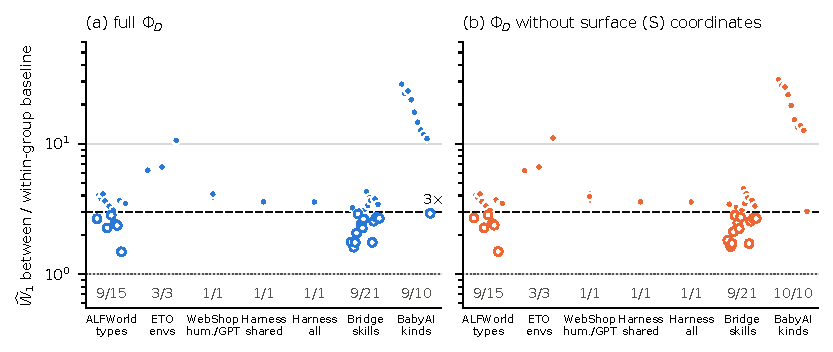
\includegraphics[width=\textwidth]{figures/fig_c2.pdf}
\caption{Structural shift between groups of reference trajectories (Experiment~2). Vertical axis: ratio $R$ of the between-group $\widehat W_1$ to the larger of the two within-group baselines, on a logarithmic scale. One marker per pair of groups, spread sideways within a column. (a) All coordinates of $\Phi_D$. (b) Without the surface coordinates (S). Columns from left to right: the six ALFWorld task types, the three ETO environments, human against GPT-4 demonstrations in WebShop (hum./GPT), SWE-agent against OpenHands, in which harness and model both differ, on the issues resolved by both (Harness shared) and on all resolved issues (Harness all), the seven Bridge skills and the five BabyAI instruction kinds. Filled marker: separated pair. Hollow marker: pair not separated. Dashed line, labelled $3\times$: $R=3$. Dotted line: $R=1$. Bars: standard deviation over seeds of the between-group $\widehat W_1$, divided by the larger baseline; most are hidden by the markers. Numbers at the bottom: separated pairs out of all pairs of the column.}
\label{fig:c2}
\end{figure}

Figure~\ref{fig:c2} shows $R$ for all pairs. Of the $52$ pairs, $33$ are separated, and all coefficients of variation are at most $0.095$. The separated pairs include all three pairs of ETO environments ($R=6.26$--$10.60$), nine of the ten BabyAI pairs ($10.94$--$28.65$), the pair of human and GPT-4 demonstrations ($4.11$), both code-agent pairs ($3.58$) and $9$ of the $15$ ALFWorld pairs. Pairs whose tasks share a sequence of subgoals stay below $R=3$, such as heating against cooling an object in ALFWorld ($1.48$, the smallest ratio of all pairs) and put next to against a pick-up followed by a go-to in BabyAI ($2.92$). In BridgeData $9$ of the $21$ pairs are separated: the demonstrations of one skill vary widely, and the large baselines ($1.23$--$1.99$, against at most $1.39$ for ALFWorld and $0.61$ for ETO) lower $R$. Without the surface coordinates (panel b), $34$ pairs are separated. The estimate $\widehat W_1$ on $\Phi_D$ thus separates $33$ of the $52$ pairs of groups of reference trajectories, among them most of those that differ in environment, instruction kind or demonstrator, and it estimates the distance $W_1(\nu_S,\nu_T)$ of the shift term.

\subsubsection{Experiment 3: One Model in Two Agent Harnesses}
\label{app:c2-harness}

The code-agent pairs of Experiment~2 change the harness and the model together. Experiment~3 holds the model fixed, changes only the harness, and compares the model's own episodes, which are the trajectories that run-time monitors, verifiers and trajectory filters read. We run Qwen3-8B \citep{qwen2025qwen3}, an open-weight model with eight billion parameters, in bf16 with its thinking mode disabled, served by vLLM \citep{kwon2023vllm} in two harnesses with the same sampling settings (temperature $0.7$, top-$p$ $0.8$, top-$k$ $20$, at most $4{,}096$ tokens per response) and at most $100$ model calls per episode: mini-SWE-agent 2.4.6 \citep{yang2024sweagent}, which gives the model a single shell tool, and OpenHands, which has separate tools for shell commands and for viewing and editing files. The tasks are $300$ of the $500$ instances of SWE-bench Verified \citep{jimenez2024swebench,openai2024swebenchverified}, human-checked GitHub issues of Python repositories, drawn in proportion to the number of instances per repository. Each instance is run once in each harness, in a fresh container built from the official image of the instance. We project the episodes onto the $16$ coordinates of the code-agent projection of Experiment~2 and compute $R$ with ten seeds and $N=150$, half the episodes of each harness.

Between the harnesses $\widehat W_1=3.81$, with a coefficient of variation of $0.024$, against baselines of $1.48$ for mini-SWE-agent and $1.74$ for OpenHands, so $R=2.19$. Computed on each coordinate alone, $\widehat W_1$ between the harnesses exceeds that coordinate's own baseline by a factor of $1.95$ to $11.5$. The largest differences concern reading code, where the harnesses offer different tools. Under mini-SWE-agent the model makes $50.4$ read calls per episode against $17.3$ under OpenHands and $73.8$ tool calls in all against $43.5$. The success changes as well. On the $299$ instances whose reference fix passes the tests, the resolve rate rises from $1.7\%$ under mini-SWE-agent to $6.4\%$ under OpenHands, by $4.7$ points (95\% confidence interval $[2.0,7.7]$, McNemar test $p=0.001$).

Changing the harness alone thus moves the trajectories of Qwen3-8B along every coordinate and changes how often the agent succeeds, so a monitor, verifier or trajectory filter calibrated on one harness receives shifted inputs under the other.

\subsection{Lemma~\ref{lemma:ape_shattering} under Shifted Position Indices}
\label{app:c1}

Lemma~\ref{lemma:ape_shattering} states that shifting the position indices of a sub-trajectory changes the attention scores of an APE model almost surely, while under RoPE they stay the same (Appendix~\ref{app:proof-rope-equivariance}). APE adds a learned vector for each position to the embedding of the token at that position (Appendix~\ref{app:attention-translation}), RoPE \citep{su2023roformerenhancedtransformerrotary} rotates queries and keys so that a score depends on the positions only through their distance, and ALiBi \citep{press2022trainshorttestlong} subtracts from each score a slope per head times the distance. Experiments~4--6 shift all position indices without inserting a token, so the tokens and their distances stay the same, and in exact arithmetic every attention score under RoPE and every attention weight under ALiBi is unchanged.

Experiments~4 and~5 use $33$ public base models, trained only to predict the next token. Twelve use APE: GPT-2 \citep{radford2019language} with 124M to 1.5B parameters, GPT-Neo \citep{black2021gptneo} with 125M to 2.7B and OPT \citep{zhang2022opt} with 125M to 6.7B. Five use ALiBi: BLOOM \citep{bigscience2022bloom} with 560M to 7.1B. Sixteen use RoPE: six Pythia models \citep{biderman2023pythia} with 160M to 6.9B, GPT-J 6B \citep{wang2021gptj}, OLMo-2 \citep{olmo2024olmo2} with 1B and 7B, SmolLM2 \citep{allal2025smollm2} with 135M to 1.7B, and Qwen2.5 \citep{qwen2024qwen25} with 0.5B to 7B.

\subsubsection{Experiment 4: Attention Scores of Pretrained Models}
\label{app:c1-kernel}

Experiment~4 compares the attention scores of full pretrained architectures with and without a shift of all position indices, to test whether those of APE models change substantially and those of RoPE models stay unchanged up to rounding. We use eight of the $33$ models: GPT-2 124M and 355M and GPT-Neo 125M and 1.3B with APE, and Pythia 160M, 410M and 1.4B and SmolLM2 360M with RoPE. Each model reads $512$ sequences of $512$ tokens, $128$ from each of four families: Countdown reference trajectories of $\mu_{DFS}$ and of $\mu_{BFS}$, Dyck-$4$ strings of four kinds of brackets nested at most $12$ deep, and source files of the Python 3.10 standard library \citep{cpython31019}. Each sequence runs once with position indices $0,\dots,511$ and once with $k,\dots,511+k$ for $k\in\{16,64,256\}$, within the context of every model ($96$ combinations of model, shift and family). All runs are in fp32 with the TF32 mode of the GPU turned off, and each is repeated in float64 to separate real changes from rounding. We record the largest change of the attention scores before the softmax, divided by the largest absolute score, in the first layer and over all layers, the share of positions whose top-1 next-token prediction changes, and the change of the log-likelihood of the text in nats per token.

In all $48$ combinations with an APE model, the largest first-layer change is $0.42$--$1.19$ of the largest absolute score, the same order as the scores themselves. The shift changes $14.0$--$87.4\%$ of the top-1 predictions and lowers the log-likelihood by $0.20$--$6.77$ nats per token. Under RoPE the change in fp32 is at most $6.2\times10^{-6}$ in the first layer and $3.2\times10^{-3}$ over all layers, of the same order as the difference between the fp32 and float64 computations without any shift, and in float64 it is at most $4.4\times10^{-12}$, so the fp32 change is rounding. RoPE changes at most $0.038\%$ of the top-1 predictions, all at near-ties between the two most likely tokens. The contrast of Lemma~\ref{lemma:ape_shattering} thus holds in the attention scores and predictions of these eight pretrained models.

\subsubsection{Experiment 5: Answers under Shifted Position Indices}
\label{app:serving}

Experiment~5 applies the shifts of position indices that occur when a model is served (through padding, cached prefixes and sliding windows) and checks whether they change the answers of APE models and leave those of RoPE and ALiBi models unchanged. Each of the $33$ models answers $3{,}000$ items, scored by exact match: $500$ for each of five few-shot tasks (copying $6$--$24$ words, reversing $2$--$4$ words, closing a Dyck-$4$ prefix, adding two numbers of $1$--$2$ digits, and completing a line of a Countdown search trace) and $500$ key--value retrieval items whose prompts grow with the context of the model, up to $3{,}000$ tokens. Decoding is greedy with cached keys and values, in fp32 except in condition (vi) below, and each item is decoded in the same batch as its unshifted version.

We shift the position indices by $k\in\{16,64,256,1024\}$, within the trained context, in four ways that occur in serving: (i) all indices; (ii) left padding with $k$ tokens and position indices that count the padding; (iii) a cached prefix, the prompt up to its final question, computed $k$ positions later; and (iv) a sliding window with attention sinks \citep{xiao2024streamingllm}, which keeps the $128$ most recent cache slots and the first four, shifted by $k$ and compared with the same window without the shift (few-shot tasks only). In the control (v), a cached prefix of $P$ tokens keeps its indices and the rest of the prompt starts at $P+k$, so every distance between the prefix and a later token grows by $k$. Condition (vi) repeats (i) in bf16. A change in accuracy is significant when its paired bootstrap 95\% confidence interval over items excludes $0$.

\begin{figure}[t]
\centering
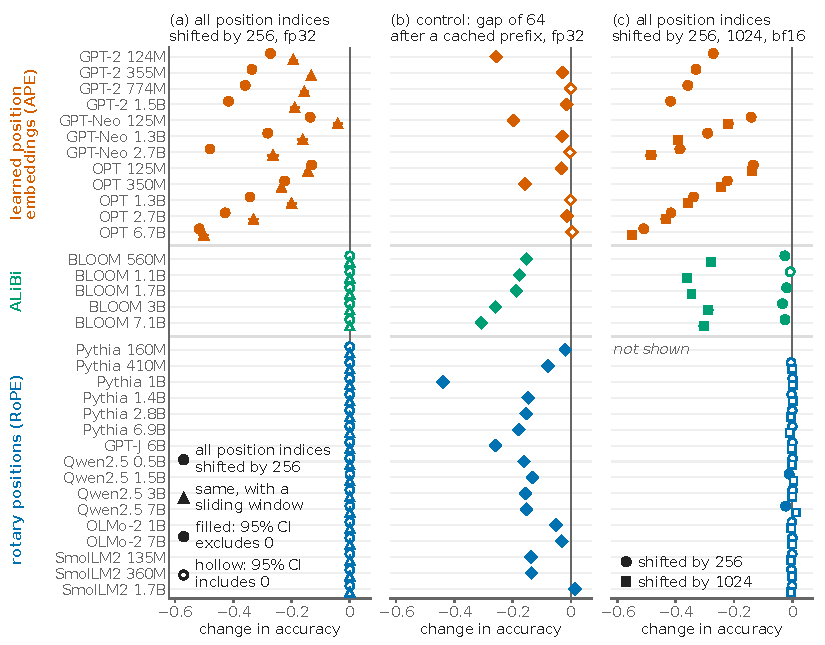
\includegraphics[width=\textwidth]{figures/fig_shift.pdf}
\caption{Change in accuracy caused by shifting the position indices, for the $33$ models of Experiment~5, one row per model, grouped and colored by positional encoding (APE, ALiBi, RoPE). Horizontal axis: accuracy with the shift minus accuracy without it. Bars: paired bootstrap 95\% confidence intervals over items, mostly hidden by the markers. Filled marker: the interval excludes $0$. Hollow marker: it includes $0$. (a) fp32. Circles: all position indices shifted by $256$, condition (i). Left padding (ii) and a cached prefix placed $256$ positions later (iii) give the same changes for the APE models and changes of at most $0.0003$ for the others, and are not drawn. Triangles: the same shift inside a sliding window (iv), compared with the sliding window without the shift (few-shot tasks only). (b) Control (v), fp32, diamonds: the cached prefix keeps its position indices and the rest of the prompt starts $64$ positions later. (c) bf16: all position indices shifted by $256$ (circles) and by $1024$ (squares, where the shifted prompt fits the trained context). Pythia 160M is not shown in (c), since its bf16 accuracy without the shift is $0.012$.}
\label{fig:shift}
\end{figure}

Figure~\ref{fig:shift} shows the results. In fp32 under (i)--(iv), the $21$ ALiBi and RoPE models change $40$ of their $948{,}000$ answers, and every accuracy changes by at most $0.0003$. The twelve APE models lose $0.13$--$0.52$ in accuracy at $k=256$ under (i)--(iii) and $0.04$--$0.50$ under (iv), and under (i) at $k=256$ they change $70$--$100\%$ of their answers. In the control (v), the answers change under all three encodings, by up to $0.44$ in accuracy at $k=64$, and the change is significant for $63$ of the $64$ combinations of RoPE model and shift and for $19$ of the $20$ of ALiBi model and shift. In bf16 the APE losses remain. The RoPE models other than Pythia 160M (not shown in Figure~\ref{fig:shift}c) stay within $0.022$ of their unshifted bf16 accuracy, with significant changes only for Qwen2.5 1.5B and 7B at $k\ge64$. The ALiBi models lose $0.007$--$0.033$ at $k=256$ and $0.28$--$0.36$ at $k=1024$, consistent with BLOOM adding the slope times the absolute position of the key, which equals the slope times the distance up to one constant per query but has a bf16 rounding error that grows with the position index. The shifts of position indices that occur in serving thus change the answers of the APE models, while the ALiBi and RoPE models in fp32 keep theirs as long as the distances between tokens are kept.

\subsubsection{Experiment 6: Two Countdown Models of Section~\ref{sec:experiments}}
\label{app:g1}

Experiment~6 turns to the two models of Appendix~\ref{app:gbc_check}, $f_1$ (RoPE, $L=12$) and $f_2$ (APE, $L=48$): we shift all their position indices in fp32 and record the effect on their routing decisions and their success on Countdown. The routing decisions are the node identifier after \texttt{Moving to Node} and the operation after \texttt{Exploring Operation} (Appendix~\ref{app:countdown_example}). We use those after the first leaf-level operation line of each trajectory, a line that explores an operation on a node with two numbers, such as \texttt{Exploring Operation: 3+10=13, Resulting Numbers: [13]}. After this line the model must decide where the search goes next. The line comes before the end of the search and directly after a dead end at the same node or a return to that node, and the node still has an unexplored operation whose result misses the target. In the teacher-forced test, the model reads a reference trajectory, and we compare its routing predictions after this line with and without a shift of all position indices by $16$ or $64$. In the free-running test, the model generates its own trajectory, generation resumes at this line with all indices shifted by $16$ or $64$, and the outcome is scored as in Section~\ref{sec:experiments}.

On the $2{,}863$ reference trajectories of the three evaluation sets in which such a line, followed by at least one routing decision, lies within the first $896$ tokens, the shift changes none of the $94{,}278$ routing predictions of the RoPE model, and $25.7\%$ (shift $16$) and $28.3\%$ (shift $64$) of those of the APE model. The free-running test uses the first $1{,}000$ problems of each evaluation set and applies to the $2{,}128$ problems for the RoPE model and the $1{,}143$ for the APE model whose output contains such a line with at least $64$ of the $512$ tokens of the generation budget left. For the RoPE model the outcome of none of these problems changes (success $0.594$). For the APE model, success falls from $0.527$ by $0.40$ (shift $16$) and by $0.39$ (shift $64$). The contrast of the lemma thus carries over to the task success of two models of the paper, consistent with the mechanism of Assumption~\ref{assum:ar_sensitivity}, in which changed routing decisions turn into failed searches.

\subsection{Splitting Deeply Nested Tasks into Separate Model Calls}
\label{app:handoff}

Lemma~\ref{lemma:dyck_homomorphism} maps a Countdown search to a word of brackets, and any task with nested subgoals can be written in the same way. Lemma~\ref{lemma:depth_bottleneck} bounds the risk from below when the nesting that one forward pass must resolve exceeds $\alpha_{\mathrm{circ}}L$, which gives the depth term. Agent systems often spread deep nesting over several calls, for example by passing a subtask to a sub-agent. Experiments~7 and~8 measure whether such splitting restores success and how deep each call should be.

In such a word, \texttt{( a} opens a subgoal of type \texttt{a} and \texttt{) a} closes it, and at every closing bracket the model predicts the type that is closed. With calls of depth at most $2$, the plan \texttt{( a ( b ( c ( d ) d ) c ) b ) a} becomes the call \texttt{( a ( b ) b ) a}, in which \texttt{b} is an empty subgoal, followed by \texttt{( b ( c ) c ) b} and \texttt{( c ( d ) d ) c}, each in a fresh context. A task is solved only if every prediction of every call is correct, and the program that splits the task uses only its nesting structure. On a calibration set, separate from the test set, we measure how often one call solves a task of each depth, fit to these rates a curve that does not increase with depth, and read from it $d_{\mathrm{ext}}$, the largest depth at which one call succeeds at least half the time, and $\hat d$, the largest depth at which it succeeds at least $80\%$ of the time. Figure~\ref{fig:split} shows the results.

\begin{figure}[!htbp]
\centering
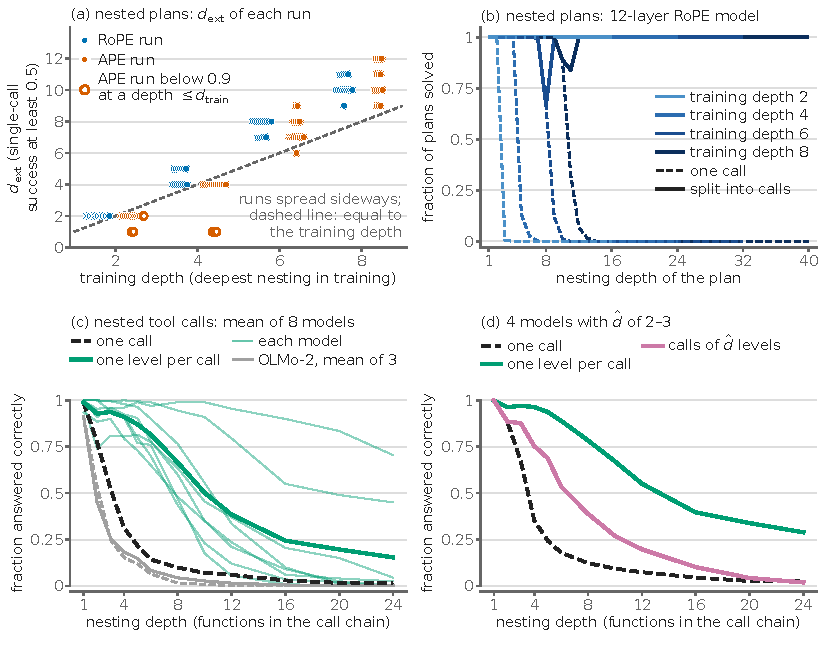
\includegraphics[width=\textwidth]{figures/fig_split.pdf}
\caption{Splitting deeply nested tasks into separate model calls (Experiments~7 and~8). (a) Experiment~7: $d_{\mathrm{ext}}$, the largest depth that one call solves at least half the time, for each of the $120$ runs (vertical axis), against the training depth $d_{\mathrm{train}}$ (horizontal axis). RoPE runs are drawn left and APE runs right of each training depth, and runs with equal values are spread sideways. Dashed line: $d_{\mathrm{ext}}=d_{\mathrm{train}}$. Hollow markers: the six runs of the two-layer width-$624$ APE model at $d_{\mathrm{train}}=2$ and $4$, whose single-call success stays below $0.9$ at some depth up to $d_{\mathrm{train}}$. (b) Experiment~7, 12-layer RoPE model: fraction of plans solved (mean of $3$ seeds) against the nesting depth of the plan, one shade per training depth. Dashed: one call. Solid: plans deeper than $d_{\mathrm{ext}}$ split into calls of depth $\min(d_{\mathrm{ext}},d_{\mathrm{train}})$, and other plans solved in one call. The dips between $d_{\mathrm{train}}$ and $d_{\mathrm{ext}}$ come from plans that are still solved in one call. (c, d) Experiment~8: fraction of the $200$ test chains answered correctly against the depth $d$, the number of functions in the chain. (c) Mean of the eight Qwen, Phi and Mistral models with one call (dashed) and with one level per call (thick solid green). Thin lines: each of these models with one level per call. Gray, with the same line styles: mean of the three OLMo-2 models. (d) Mean of the four models whose $\hat d$ is $2$ or $3$: one call (dashed), one level per call (green) and calls of $\hat d$ levels (pink).}
\label{fig:split}
\end{figure}

\subsubsection{Experiment 7: Nested Plans}
\label{app:nestplan}

Experiment~7 trains small models from scratch on nested plans to test whether splitting restores success beyond $d_{\mathrm{ext}}$, and whether $d_{\mathrm{ext}}$ follows the number of layers, as the threshold $\alpha_{\mathrm{circ}}L$ suggests, or the depth of the training plans. A plan has $48$ subgoals of $8$ types and maximum nesting depth exactly $d$: a spine of $d$ nested subgoals and $48-d$ further subgoals, each attached at random to a subgoal of depth below $d$ or to the top level. Every plan has $194$ tokens regardless of its depth, and it is solved when the type predicted at each of its $48$ closing brackets is correct, all other tokens being given.

We train the GPT-NeoX (RoPE) and GPT-Neo (APE) architectures of Appendix~\ref{app:reproducibility} in five shapes, width $256$ with $L\in\{2,4,8,12\}$ layers and a two-layer model of width $624$ whose number of parameters matches that of the 12-layer model within $1.3\%$, on plans whose depth is drawn uniformly from $1$ to $d_{\mathrm{train}}\in\{2,4,6,8\}$. Training takes $30{,}000$ steps of $256$ plans (AdamW, peak learning rate $10^{-3}$ with cosine decay, loss on the predicted types), and the $40$ configurations (two encodings, five shapes, four training depths) with three seeds each give $120$ runs. Five configurations in which some run stays below a single-call success of $0.9$ at a depth up to $d_{\mathrm{train}}$ are trained again for $60{,}000$ steps, after which three of them reach $0.9$ at every such depth in every run. For each run, $d_{\mathrm{ext}}$ comes from $200$ calibration plans per depth. A plan deeper than $d_{\mathrm{ext}}$ is split into calls of depth $D=\min(d_{\mathrm{ext}},d_{\mathrm{train}})$, which keeps every call within the training depths and needs $D\ge2$. The test sets have $500$ plans per depth, up to depth $4d_{\mathrm{train}}+8$.

In $38$ of the $40$ configurations, every run reaches a single-call success of at least $0.9$ at every depth up to $d_{\mathrm{train}}$. In all $114$ runs of these configurations, splitting gives a mean success of at least $0.987$ over the depths beyond $d_{\mathrm{ext}}$, and at least $0.91$ at each of them, against at most $0.04$ for one call, as Figure~\ref{fig:split}b shows for the 12-layer RoPE model. $d_{\mathrm{ext}}$ follows $d_{\mathrm{train}}$: it is $2$, $4$--$5$, $6$--$9$ and $9$--$12$ for $d_{\mathrm{train}}=2$, $4$, $6$ and $8$, with no systematic dependence on the number of layers, the width or the positional encoding, and exceeds $d_{\mathrm{train}}$ by at most four levels (Figure~\ref{fig:split}a). Training on deeper plans reduces the number of calls: beyond $d_{\mathrm{ext}}$, a plan needs $20.8$ calls on average at $d_{\mathrm{train}}=2$ and $4.5$--$4.6$ at $d_{\mathrm{train}}=8$. The two other configurations are the two-layer width-$624$ APE model at $d_{\mathrm{train}}=2$ and $4$: five of their six runs have $d_{\mathrm{ext}}=1$, too shallow for a split with $D\ge2$, and in the sixth splitting raises the success beyond $d_{\mathrm{ext}}=2$ from $0.00$ to $0.998$. In models of $2$ to $12$ layers, the depth that one call resolves thus follows the training depth independently of $L$, and splitting into calls within the training depths restores success on deeper plans.

\subsubsection{Experiment 8: Nested Tool Calls with Open-Weight Language Models}
\label{app:llm-handoff}

Experiment~8 measures $\hat d$ for pretrained language models, whose training depth is unknown, on a task shaped like the tool calls of an agent: a registry lists one-line Python functions, and a question asks for the value of a chain of nested calls, such as \texttt{bell(4)} for the registry
{\footnotesize
\begin{verbatim}
def lamp(x): return x + 2
def door(x): return lamp(x) + 3
def bell(x): return door(x) + 1
\end{verbatim}
}
\noindent a chain of depth $d=3$ whose value is $10$. With one level per call, the chain is split from the innermost function outward: the first call returns $\texttt{lamp(4)}=6$, and the next call sees the line of \texttt{lamp} replaced by this value and asks for \texttt{door(4)}. Only the answer of the last call is scored.

A registry has $26$ lines: the $d$ functions of the chain, named by common English nouns and each adding a constant $c\in\{1,2,3\}$, two distractor functions, and $24-d$ comment lines that keep the length of the prompt the same for every $d$. Four worked examples precede every prompt. The model may generate at most eight tokens, and the first integer among them is scored by exact match, so the model must follow the chain within its forward passes. The calibration set has $100$ and the test set $200$ items for each $d\in\{1,2,3,4,5,6,8,10,12,16,20,24\}$. We evaluate eleven instruction-tuned models in bf16 with greedy decoding: Qwen2.5 \citep{qwen2024qwen25} (7B, 14B and 32B parameters), OLMo-2 \citep{olmo2024olmo2} (7B, 13B, 32B), Qwen3 \citep{qwen2025qwen3} (8B, 14B, 32B, thinking mode disabled), Phi-4 14B \citep{abdin2024phi4} and Mistral-Small-24B-Instruct-2501 \citep{mistral2025small3}. We compare four ways of answering: one call; one call whose prompt also lists the open call chain, such as \texttt{bell(4) -> door(4) -> lamp(4)}; one level per call, with $d$ calls; and calls of $\hat d$ levels, with $\lceil d/\hat d\rceil$ calls and $\hat d$ measured for each model on the calibration set.

The accuracy of one call falls quickly as the chain grows (Figure~\ref{fig:split}c), from $0.88$--$1.00$ at $d=1$ to at most $0.52$ at $d=4$ and at most $0.15$ at $d=8$. $\hat d$ is $3$ for Qwen2.5 32B, $2$ for Qwen3 14B, Phi-4 and Mistral-Small-24B, and $1$ for the other seven models. Listing the chain changes the single-call accuracy by at most $0.09$ on average over depths. One level per call raises the accuracy of the eight Qwen, Phi and Mistral models at $d=8$ from $0.01$--$0.15$ to $0.43$--$0.99$, and Mistral-Small-24B answers $0.70$ of the chains correctly at $d=24$. For the three OLMo-2 models, one level per call gives $0.04$--$0.06$ at $d=8$, against $0.00$--$0.03$ in one call, and $0.37$--$0.59$ at $d=2$, against $0.43$--$0.72$. For the four models whose $\hat d$ is $2$ or $3$ (Figure~\ref{fig:split}d), calls of $\hat d$ levels need $4$ or $3$ calls at $d=8$ and reach $0.24$--$0.51$, against $0.43$--$0.99$ with one level per call. Every call after the first uses the value returned by the previous call, so the errors of the calls compound, and by the definition of $\hat d$ a call of $\hat d$ levels errs in up to a fifth of the cases. One level per call therefore outperforms calls of $\hat d$ levels at $d=8$ for all four models where the two differ, since each of its calls stays at a depth where a single call is almost always correct.

\clearpage
\subsection{Summary of the Eight Experiments}
\label{app:uses}

Table~\ref{tab:apps} summarizes the eight experiments. Each concerns one part of Theorem~\ref{thm:unified_bound}: Experiment~1 the balance between the residual $\epsilon$ and the estimation of $W_1$, Experiments~2 and~3 the distance $W_1$ in the shift term, Experiments~4--6 the factor $K_{f,\mathrm{PE}}$ through Lemma~\ref{lemma:ape_shattering}, and Experiments~7 and~8 the depth term.

\begin{table}[!h]
\centering\footnotesize
\setlength{\tabcolsep}{3pt}
\caption{Results of the eight experiments of Appendix~\ref{app:beyond}. \emph{Experiment}: number, short name and section. \emph{Setting}: the models and data. \emph{Finding}: the main numbers and what they show.}
\label{tab:apps}
\begin{tabular}{@{}p{0.20\linewidth}p{0.28\linewidth}p{0.48\linewidth}@{}}
\toprule
\ontoR\textbf{Experiment} & \ontoR\textbf{Setting} & \ontoR\textbf{Finding} \tabularnewline
\midrule
\ontoR 1. More coordinates on Countdown (\ref{app:refine}) & \ontoR 12, 16, 24 and 34 coordinates; $f_1$ and $f_2$; training trajectories of the three measures & \ontoR ROC-AUC changes by at most $0.003$, while $\widehat W_1$ between measures grows by a factor of $1.8$--$2.0$; the twelve coordinates are the better choice \tabularnewline
\ontoR 2. Groups of agent, embodied and robot trajectories (\ref{app:c2-groups}) & \ontoR $52$ pairs of groups from the ETO expert trajectories, the Nebius code-agent runs, BridgeData V2 and BabyAI & \ontoR $33$ pairs separated ($34$ without surface coordinates); tasks that share a sequence of subgoals give the smallest ratios \tabularnewline
\ontoR 3. One model in two agent harnesses (\ref{app:c2-harness}) & \ontoR Qwen3-8B in mini-SWE-agent and OpenHands, $300$ SWE-bench Verified instances & \ontoR $R=2.19$, and every coordinate moves by $1.95$--$11.5$ times its own baseline; the resolve rate rises from $1.7\%$ to $6.4\%$ \tabularnewline
\ontoR 4. Attention scores of pretrained models (\ref{app:c1-kernel}) & \ontoR Four APE and four RoPE models; shifts of $16$, $64$ and $256$ & \ontoR Under APE the first-layer change is $0.42$--$1.19$ of the largest score; under RoPE the change is rounding (at most $4.4\times10^{-12}$ in float64) \tabularnewline
\ontoR 5. Answers under shifted position indices (\ref{app:serving}) & \ontoR $33$ public models; all indices shifted, left padding, cached prefix, sliding window & \ontoR In fp32 the ALiBi and RoPE models change $40$ of $948{,}000$ answers, and the APE models lose $0.13$--$0.52$ in accuracy at $k=256$; a gap after a cached prefix changes the answers under every encoding \tabularnewline
\ontoR 6. Two Countdown models (\ref{app:g1}) & \ontoR $f_1$ (RoPE) and $f_2$ (APE) of Section~\ref{sec:experiments} & \ontoR No outcome of the RoPE model changes; the success of the APE model falls by $0.40$ and $0.39$ (shifts $16$ and $64$) \tabularnewline
\ontoR 7. Nested plans (\ref{app:nestplan}) & \ontoR $120$ runs ($40$ configurations, three seeds) trained from scratch, $d_{\mathrm{train}}\in\{2,4,6,8\}$ & \ontoR In the $114$ runs that learned their training depths, splitting gives a mean success of at least $0.987$ beyond $d_{\mathrm{ext}}$, against at most $0.04$ for one call; $d_{\mathrm{ext}}$ follows $d_{\mathrm{train}}$ \tabularnewline
\ontoR 8. Nested tool calls (\ref{app:llm-handoff}) & \ontoR $11$ open-weight models of 7B--32B parameters & \ontoR With one level per call, the accuracy of eight models at $d=8$ rises from $0.01$--$0.15$ to $0.43$--$0.99$; calls of $\hat d$ levels reach $0.24$--$0.51$ \tabularnewline
\bottomrule
\end{tabular}
\end{table}
\clearpage
